\section{Introduction}\label{sec:1}

Current multimodal systems implement vision, audio, and text through separately-designed neural encoders: a ViT image branch~\cite{ref2}, a Whisper audio branch~\cite{ref3}, and a GPT-class text decoder~\cite{ref4}, connected via learned projection layers at fusion points. \QC{}~\cite{ref1} replaces the per-modality design with a single sequence-mixing primitive grounded in the reinforcement-learning $Q$-function: the same primitive, differing only in whether a causal mask is applied, is used for all four modalities. Standard attention variants~\hyperlink{cite.ref5}{5}--\hyperlink{cite.ref9}{9} retain the four-projection $QKVO$ structure and are typically optimized as a separate encoder per modality. \QC{} drops the value projection $W_V$ and scores attention via a $Q$-function over learned state/action projections.

This paper is the empirical follow-up to~\cite{ref1}. It introduces two extensions deferred in that work and evaluates them at three parameter scales (57M, 121M, 179M) on four modalities. The central claims are:

\begin{enumerate}[leftmargin=*,labelindent=\parindent,itemsep=0.6ex]
\item \textbf{SAVO closes most of the SAO$\to$QKVO 60m text-LM gap.} The four-projection variant in which the $V$ projects the state$\odot$action product reduces the perplexity gap from 20 ppl to $+12.33 \pm 0.87$ ppl at 60m (4-seed paired-difference vs the rank-matched controlled ablation, $p = 7.6 \times 10^{-4}$). A comparable ${\sim}$11-ppl gap holds at 120m and 180m (single seed each, magnitude consistent with the 60m multi-seed mean).
\item \textbf{Cross-modal non-interference is empirical, not assumed.} At matched text compute, joint four-modality training at 60m reaches the same per-text-token loss as text-only training; the property holds through 180m.
\item \textbf{World-model concurrent with text/vision/audio.} The world objective trains stably alongside the other three modalities (MSE $1.125 \to 0.071$ over the 10,000-step budget); MiniGrid-Empty-8x8's low next-state variance puts the predict-mean baseline (0.033) in the same band as the trained TransitionModel, so the routing primitive's concurrent multimodal capacity --- not world-model dominance --- is what we report.
\item \textbf{Cross-field demonstration.} The same SAVO block class trains on four computational-oncology tasks (signature decomposition, pan-cancer classification, drug-response regression, 5-year survival prediction). Per-task performance ranges from competitive (Phase 3 GDSC drug-response, $r{=}0.903$) to slightly below specialist baselines (Phase 1 NNLS, Phase 4 clinical-only), indicating the routing primitive trains and converges across these domains; per-domain superiority is not claimed.
\end{enumerate}

The work is purely empirical. The architectural primitive and its theoretical justification are established in~\cite{ref1}; here we ask how it behaves at scale across modalities and where the boundaries of its current evaluation lie.

\section{Related Work}\label{sec:2}

\paragraph{Attention variants.} Numerous works modify the attention mechanism while retaining the QKVO four-projection structure: linear attention~\cite{ref6}, sparse attention~\cite{ref7}, FlashAttention~\cite{ref8}, and grouped-query attention~\cite{ref9}. None eliminate $W_V$ as an architectural decision. \QC{}~\cite{ref1} does, grounding the removal in $Q$-function theory; the four-projection variant introduced here (\S\ref{sec:3.1}) reintroduces a $V$, but the $V$ projects the state-action product, not the raw input.

\begin{figure}[H]
\centering
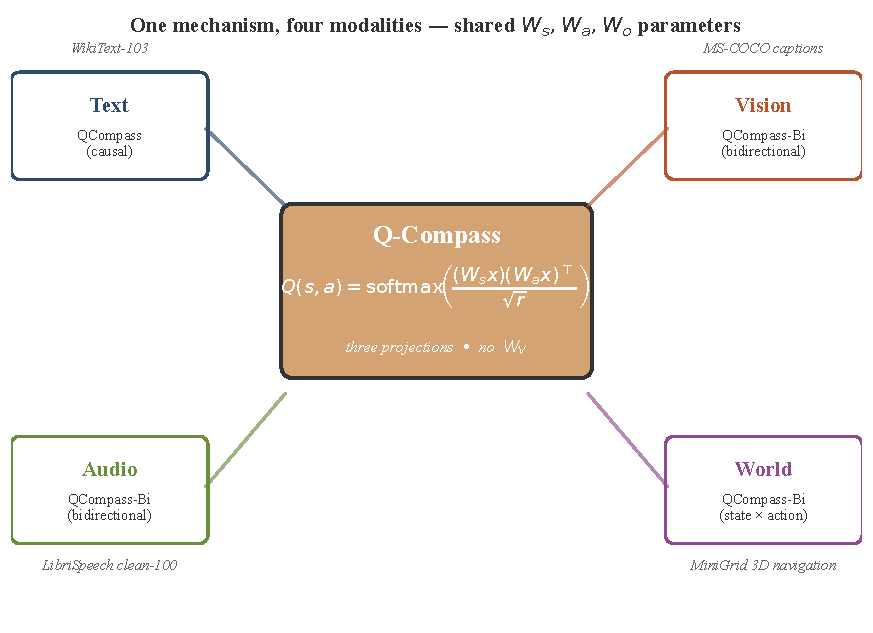
\includegraphics[width=.929\linewidth]{figs/fig01.pdf}
\caption{\textbf{One mechanism, four modalities.} The same \QCBi{} block implements routing for text, vision, audio, and world-model pipelines. Text uses the causal variant (\QC{}); all other modalities use the bidirectional variant (\QCBi{}). The $W_s, W_a, W_o$ projection matrices are structurally identical across pipelines; only dimensionality and layer count vary per modality.}
\label{fig:1}
\end{figure}

\paragraph{Multimodal architectures.} Current systems compose modality-specific encoders: ViT~\cite{ref2} and CLIP~\cite{ref10} for vision; Whisper~\cite{ref3} for audio; GPT-class decoders~\cite{ref4} for text. Flamingo~\cite{ref11} fuses them via learned cross-attention. Perceiver IO~\cite{ref12} introduces a shared latent bottleneck but retains standard attention. Gato~\cite{ref13} tokenizes multiple modalities into a common embedding space for a single transformer decoder; the attention kernel inside Gato is still QKVO, and unification occurs at the tokenization layer rather than at the routing primitive.

\paragraph{World models.} Ha and Schmidhuber~\cite{ref14} and the Dreamer lineage~\cite{ref15} established the state--action--transition decomposition we adopt. We parameterize all three components (StateEncoder, TransitionModel, ActionHead) using \QCBi{} blocks. Our objective here is to test that the routing primitive supports a world-model objective concurrently with text/vision/audio inside a single shared backbone --- not to benchmark against dedicated world-model architectures, for which target-network EMAs, predictor heads, contrastive auxiliaries, and richer environments (DMLab, Habitat) are the standard ingredients.

\section{Method}\label{sec:3}

We use \QC{}~\cite{ref1} as the routing primitive throughout. Given input $x \in \mathbb{R}^{B\times L\times H}$, \QC{} computes $\text{state} = xW_s$, $\text{action} = xW_a$ (both $\in \mathbb{R}^{B\times L\times r}$), $Q(s,a) = \operatorname{softmax}((\text{state}\cdot\text{action}^{\top})/\sqrt{r} + M)$, and $\text{output} = W_o(Q(s,a)\cdot x)$, where $M$ is an optional causal mask. Mechanism, parameter accounting, and the bidirectional variant (\QCBi{}, $M=0$) are described in the original paper. The remainder of this section introduces two architectural variants deferred in~\cite{ref1} and the modality pipelines. Of the two, only SAVO ($W_c$ $Q$-value content) closes the SAO$\to$QKVO text-LM gap; multi-head \QC{} (MH-QC) is a null result we report transparently in \S\ref{sec:5.7}.

\subsection{SAVO: a four-projection \QC{} with $Q$-value content}\label{sec:3.1}

Vanilla \QC{} (the SAO form: state, action, output) gathers raw $x_j$ as content. The SAVO variant replaces this with the token's own self-$Q$-value:
\begin{align}
\text{qval}_i &= \text{state}_i \odot \text{action}_i \qquad \in \mathbb{R}^{r} \label{eq:1}\\
\text{content}_i &= \text{qval}_i \cdot W_c \qquad (W_c \in \mathbb{R}^{r\times H}) \label{eq:2}\\
\text{output} &= W_o\bigl(Q(s,a)\cdot \text{content}\bigr). \label{eq:3}
\end{align}
The semantic reading: each token's content is the $Q$-value signature of itself as an action from its own state, computed from the same projections that drive the routing. Unlike standard attention's $W_V$, $W_c$ projects a $Q$-value (not raw $x$), so the $W_V$-free property of \QC{} is preserved at the principled level. Parameter cost: $+rH$ per block (${\sim}$18K at 60m). Since $\text{state} = xW_s$ and $\text{action} = xW_a$, SAVO's content gather $((xW_s)\odot(xW_a))W_c$ is mathematically a learned non-linear function of $x$. The ``$W_V$-free'' framing applies at the \textit{raw-input} level only --- SAVO is not free of learned content transforms; it replaces a linear projection of $x$ with a non-linear one of $(W_s, W_a, W_c)$ jointly.

\subsection{Multi-head \QC{} (MH-QC)}\label{sec:3.2}

MH-QC splits the state and action projections into $h$ heads of rank $r/h$, computes $Q^{(k)}(s,a)$ in each subspace, and concatenates the outputs:
\begin{equation}
\text{output} = W_o \cdot \bigl[Q^{(1)}\cdot x^{(1)} \,\|\, \cdots \,\|\, Q^{(h)}\cdot x^{(h)}\bigr], \label{eq:4}
\end{equation}
where $x^{(k)}$ is the $k$-th $H/h$ slice of $x$. No additional parameters: $W_s$ and $W_a$ retain their total size $H\times r$. SAVO and MH-QC compose; the combination is denoted MH-QVC. Per-block parameter counts for all four variants are listed in Table~\ref{tab:1}.

\begin{table}[H]
\centering
\small
\setlength{\tabcolsep}{3pt}
\renewcommand{\arraystretch}{1.2}
\begin{tabular*}{\linewidth}{@{\extracolsep{\fill}}lrrr}
\toprule
Variant & Attn-block params (per layer) & 60m ($H{=}384$, $r{=}48$) & 120m ($H{=}640$, $r{=}80$) \\
\midrule
\QC{} single-head (SAO) & $2Hr + H^2$ & 184,320 & 511,600 \\
MH-\QC{} (any $h$) & $2Hr + H^2$ & 184,320 & 511,600 \\
SAVO ($Q$-value content) & $3Hr + H^2$ & 202,752 & 562,800 \\
MH-QVC ($h \geq 1$, with $W_c$) & $3Hr + H^2$ & 202,752 & 562,800 \\
\midrule
Rank-matched transformer (1-head) & $4Hr$ & 73,728 & 204,800 \\
Standard multi-head attention & $4H^2$ & 589,824 & 1,638,400 \\
\bottomrule
\end{tabular*}
\caption{Per-layer attention-block parameter counts (excludes FFN, norms, embeddings). The rank-matched transformer is the apples-to-apples baseline used in \S\ref{sec:5.2}: all four projections at rank $r$, matching \QC{}'s $W_s, W_a$ rank.}
\label{tab:1}
\end{table}

\subsection{Modality pipelines}\label{sec:3.3}

\paragraph{Text (autoregressive LM).} Tokens are embedded via learned token and positional embeddings, passed through $N$ causal \textsc{QuatrixBlocks} (each a \QC{} block plus pre-norm FFN), and projected to vocabulary logits via a tied embedding head. Loss is standard next-token cross-entropy.

\paragraph{Vision.} RGB images ($224\times224$) are patchified via a $16\times16$ Conv2d into 196 patch tokens, position-embedded, passed through 3 bidirectional \QCBi{} blocks, projected to the LM hidden dimension, and prepended to the text token sequence. The joint loss is text cross-entropy over the text portion only; vision tokens do not contribute directly to the loss.

\paragraph{Audio.} Waveforms are loaded at 16\,kHz and converted to 80-mel spectrograms. The spectrogram is treated as a 2D image (frequency $\times$ time) and patchified with a $16\times16$ kernel, producing a variable number of patches. Patches are position-embedded, passed through 3 bidirectional \QCBi{} blocks, projected to the LM hidden dimension, and prepended to the text token sequence.

\paragraph{World.} Frame pairs $(\text{frame}_t, \text{frame}_{t+1})$ from MiniGrid 3D navigation trajectories are encoded via the same \textsc{VisionEncoder} used for vision training. A \textsc{StateEncoder} (a \QCBi{} block with a learnable query token prepended to the patch sequence) aggregates each frame's patches into $s_t$ or $s_{t+1}$. The discrete action ID is embedded into $a_t$. The \textsc{TransitionModel} (9--10 \QCBi{} blocks, taking the fused state-action vector as input) predicts $\hat{s}_{t+1} = \text{Transition}(s_t, a_t)$. World loss is mean squared error with the gradient through the target stopped:
\begin{equation}
\mathcal{L}_{\text{world}} = \text{MSE}\bigl(\hat{s}_{t+1},\ \text{stop\_grad}(s_{t+1})\bigr). \label{eq:5}
\end{equation}
The target detachment prevents trivial collapse via the target pathway. The world objective trains concurrently with the other three modalities; we report convergence and a comparison to the predict-mean baseline in \S\ref{sec:6.3}.

\subsection{Joint training objective and optimization}\label{sec:3.4}

At each step a single batch is sampled from one of four data loaders according to a fixed mixture (35\% text / 25\% vision / 20\% audio / 20\% world). The per-step loss is
\begin{equation}
\mathcal{L}_{\text{total}} = \alpha\,\mathcal{L}_{\text{text}} + \beta\,\mathcal{L}_{\text{vision}} + \gamma\,\mathcal{L}_{\text{audio}} + \delta\,\mathcal{L}_{\text{world}}, \label{eq:6}
\end{equation}
with $\alpha{=}\beta{=}\gamma{=}1.0$ and $\delta{=}0.5$ (world MSE on normalized state vectors has roughly $1/30$ the magnitude of text cross-entropy). We use \textbf{Muon}~\cite{ref16} for 2D linear weight matrices and \textbf{AdamW}~\cite{ref17} for embeddings, LayerNorm, and biases, with separate cosine schedules (peak Muon $3{\times}10^{-4}$, $2.5{\times}10^{-4}$, $2{\times}10^{-4}$ for 60m/120m/180m; AdamW at 1/10). The Muon Newton--Schulz orthogonalisation uses a single-stage schedule with the original~\cite{ref16} coefficients; we did not adopt the V4-style hybrid 8+2-iteration schedule~\cite{ref18} in the runs reported here. The exact iteration coefficients are pinned in the released codebase. Effective batch is 64 sequences of 1024 tokens (batch $4\times$ grad accumulation 16). Training is mixed precision (fp16 compute with loss scaling, fp32 parameters/optimizer), gradient-clipped at $\ell_2$-norm 1.0.

\begin{figure}[H]
\centering
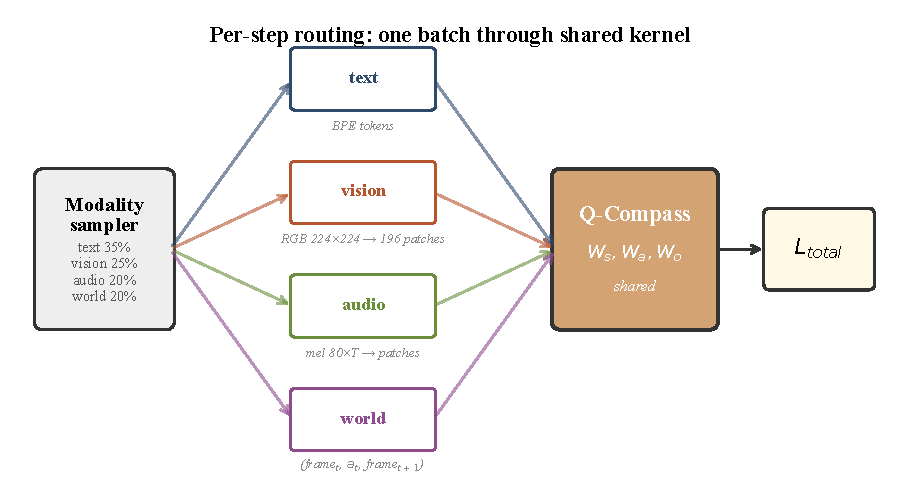
\includegraphics[width=.959\linewidth]{figs/fig02.pdf}
\caption{\textbf{Per-step routing: one batch through the shared kernel.} At each optimizer step the modality sampler draws from text (35\%), vision (25\%), audio (20\%), or world (20\%). Regardless of modality, the batch flows through the same $W_s, W_a, W_o$ parameters inside the \QC{} kernel.}
\label{fig:2}
\end{figure}
